\documentclass[twoside]{book}

% Packages required by doxygen
\usepackage{fixltx2e}
\usepackage{calc}
\usepackage{doxygen}
\usepackage[export]{adjustbox} % also loads graphicx
\usepackage{graphicx}
\usepackage[utf8]{inputenc}
\usepackage{makeidx}
\usepackage{multicol}
\usepackage{multirow}
\PassOptionsToPackage{warn}{textcomp}
\usepackage{textcomp}
\usepackage[nointegrals]{wasysym}
\usepackage[table]{xcolor}

% Font selection
\usepackage[T1]{fontenc}
\usepackage[scaled=.90]{helvet}
\usepackage{courier}
\usepackage{amssymb}
\usepackage{sectsty}
\renewcommand{\familydefault}{\sfdefault}
\allsectionsfont{%
  \fontseries{bc}\selectfont%
  \color{darkgray}%
}
\renewcommand{\DoxyLabelFont}{%
  \fontseries{bc}\selectfont%
  \color{darkgray}%
}
\newcommand{\+}{\discretionary{\mbox{\scriptsize$\hookleftarrow$}}{}{}}

% Page & text layout
\usepackage{geometry}
\geometry{%
  a4paper,%
  top=2.5cm,%
  bottom=2.5cm,%
  left=2.5cm,%
  right=2.5cm%
}
\tolerance=750
\hfuzz=15pt
\hbadness=750
\setlength{\emergencystretch}{15pt}
\setlength{\parindent}{0cm}
\setlength{\parskip}{3ex plus 2ex minus 2ex}
\makeatletter
\renewcommand{\paragraph}{%
  \@startsection{paragraph}{4}{0ex}{-1.0ex}{1.0ex}{%
    \normalfont\normalsize\bfseries\SS@parafont%
  }%
}
\renewcommand{\subparagraph}{%
  \@startsection{subparagraph}{5}{0ex}{-1.0ex}{1.0ex}{%
    \normalfont\normalsize\bfseries\SS@subparafont%
  }%
}
\makeatother

% Headers & footers
\usepackage{fancyhdr}
\pagestyle{fancyplain}
\fancyhead[LE]{\fancyplain{}{\bfseries\thepage}}
\fancyhead[CE]{\fancyplain{}{}}
\fancyhead[RE]{\fancyplain{}{\bfseries\leftmark}}
\fancyhead[LO]{\fancyplain{}{\bfseries\rightmark}}
\fancyhead[CO]{\fancyplain{}{}}
\fancyhead[RO]{\fancyplain{}{\bfseries\thepage}}
\fancyfoot[LE]{\fancyplain{}{}}
\fancyfoot[CE]{\fancyplain{}{}}
\fancyfoot[RE]{\fancyplain{}{\bfseries\scriptsize Generated by Doxygen }}
\fancyfoot[LO]{\fancyplain{}{\bfseries\scriptsize Generated by Doxygen }}
\fancyfoot[CO]{\fancyplain{}{}}
\fancyfoot[RO]{\fancyplain{}{}}
\renewcommand{\footrulewidth}{0.4pt}
\renewcommand{\chaptermark}[1]{%
  \markboth{#1}{}%
}
\renewcommand{\sectionmark}[1]{%
  \markright{\thesection\ #1}%
}

% Indices & bibliography
\usepackage{natbib}
\usepackage[titles]{tocloft}
\setcounter{tocdepth}{3}
\setcounter{secnumdepth}{5}
\makeindex

% Hyperlinks (required, but should be loaded last)
\usepackage{ifpdf}
\ifpdf
  \usepackage[pdftex,pagebackref=true]{hyperref}
\else
  \usepackage[ps2pdf,pagebackref=true]{hyperref}
\fi
\hypersetup{%
  colorlinks=true,%
  linkcolor=blue,%
  citecolor=blue,%
  unicode%
}

% Custom commands
\newcommand{\clearemptydoublepage}{%
  \newpage{\pagestyle{empty}\cleardoublepage}%
}

\usepackage{caption}
\captionsetup{labelsep=space,justification=centering,font={bf},singlelinecheck=off,skip=4pt,position=top}

%===== C O N T E N T S =====

\begin{document}

% Titlepage & ToC
\hypersetup{pageanchor=false,
             bookmarksnumbered=true,
             pdfencoding=unicode
            }
\pagenumbering{alph}
\begin{titlepage}
\vspace*{7cm}
\begin{center}%
{\Large D\+PG -\/ Fast construction of kd-\/trees based on presorting }\\
\vspace*{1cm}
{\large Generated by Doxygen 1.8.13}\\
\end{center}
\end{titlepage}
\clearemptydoublepage
\pagenumbering{roman}
\tableofcontents
\clearemptydoublepage
\pagenumbering{arabic}
\hypersetup{pageanchor=true}

%--- Begin generated contents ---
\chapter{Hierarchical Index}
\section{Class Hierarchy}
This inheritance list is sorted roughly, but not completely, alphabetically\+:\begin{DoxyCompactList}
\item \contentsline{section}{bounding\+Box}{\pageref{classbounding_box}}{}
\item \contentsline{section}{Draw\+Object}{\pageref{class_draw_object}}{}
\begin{DoxyCompactList}
\item \contentsline{section}{Sphere}{\pageref{class_sphere}}{}
\item \contentsline{section}{Triangle}{\pageref{class_triangle}}{}
\end{DoxyCompactList}
\item \contentsline{section}{Edge}{\pageref{class_edge}}{}
\item \contentsline{section}{event\+Comparator}{\pageref{structevent_comparator}}{}
\item \contentsline{section}{Image\+Structure}{\pageref{class_image_structure}}{}
\item \contentsline{section}{K\+D\+\_\+\+Tree}{\pageref{class_k_d___tree}}{}
\item \contentsline{section}{kd\+Node}{\pageref{structkd_node}}{}
\item \contentsline{section}{Material\+Base}{\pageref{class_material_base}}{}
\begin{DoxyCompactList}
\item \contentsline{section}{Material}{\pageref{class_material}}{}
\item \contentsline{section}{Material\+Emissive}{\pageref{class_material_emissive}}{}
\end{DoxyCompactList}
\item \contentsline{section}{plane\+Solution}{\pageref{structplane_solution}}{}
\item \contentsline{section}{Point\+Light}{\pageref{class_point_light}}{}
\item \contentsline{section}{Ray}{\pageref{class_ray}}{}
\item \contentsline{section}{Scene\+Structure}{\pageref{class_scene_structure}}{}
\item \contentsline{section}{split\+Plane}{\pageref{classsplit_plane}}{}
\item \contentsline{section}{Transformation\+Stack}{\pageref{class_transformation_stack}}{}
\item \contentsline{section}{triangle\+Event}{\pageref{classtriangle_event}}{}
\item \contentsline{section}{Vector3f}{\pageref{class_vector3f}}{}
\item \contentsline{section}{Vertex}{\pageref{class_vertex}}{}
\item \contentsline{section}{Voxel}{\pageref{class_voxel}}{}
\end{DoxyCompactList}

\chapter{Class Index}
\section{Class List}
Here are the classes, structs, unions and interfaces with brief descriptions\+:\begin{DoxyCompactList}
\item\contentsline{section}{\hyperlink{classbounding_box}{bounding\+Box} }{\pageref{classbounding_box}}{}
\item\contentsline{section}{\hyperlink{class_draw_object}{Draw\+Object} }{\pageref{class_draw_object}}{}
\item\contentsline{section}{\hyperlink{class_edge}{Edge} }{\pageref{class_edge}}{}
\item\contentsline{section}{\hyperlink{structevent_comparator}{event\+Comparator} }{\pageref{structevent_comparator}}{}
\item\contentsline{section}{\hyperlink{class_image_structure}{Image\+Structure} }{\pageref{class_image_structure}}{}
\item\contentsline{section}{\hyperlink{class_k_d___tree}{K\+D\+\_\+\+Tree} }{\pageref{class_k_d___tree}}{}
\item\contentsline{section}{\hyperlink{structkd_node}{kd\+Node} }{\pageref{structkd_node}}{}
\item\contentsline{section}{\hyperlink{class_material}{Material} }{\pageref{class_material}}{}
\item\contentsline{section}{\hyperlink{class_material_base}{Material\+Base} }{\pageref{class_material_base}}{}
\item\contentsline{section}{\hyperlink{class_material_emissive}{Material\+Emissive} }{\pageref{class_material_emissive}}{}
\item\contentsline{section}{\hyperlink{structplane_solution}{plane\+Solution} }{\pageref{structplane_solution}}{}
\item\contentsline{section}{\hyperlink{class_point_light}{Point\+Light} }{\pageref{class_point_light}}{}
\item\contentsline{section}{\hyperlink{class_ray}{Ray} }{\pageref{class_ray}}{}
\item\contentsline{section}{\hyperlink{class_scene_structure}{Scene\+Structure} }{\pageref{class_scene_structure}}{}
\item\contentsline{section}{\hyperlink{class_sphere}{Sphere} }{\pageref{class_sphere}}{}
\item\contentsline{section}{\hyperlink{classsplit_plane}{split\+Plane} }{\pageref{classsplit_plane}}{}
\item\contentsline{section}{\hyperlink{class_transformation_stack}{Transformation\+Stack} }{\pageref{class_transformation_stack}}{}
\item\contentsline{section}{\hyperlink{class_triangle}{Triangle} }{\pageref{class_triangle}}{}
\item\contentsline{section}{\hyperlink{classtriangle_event}{triangle\+Event} }{\pageref{classtriangle_event}}{}
\item\contentsline{section}{\hyperlink{class_vector3f}{Vector3f} }{\pageref{class_vector3f}}{}
\item\contentsline{section}{\hyperlink{class_vertex}{Vertex} }{\pageref{class_vertex}}{}
\item\contentsline{section}{\hyperlink{class_voxel}{Voxel} }{\pageref{class_voxel}}{}
\end{DoxyCompactList}

\chapter{Class Documentation}
\hypertarget{classbounding_box}{}\section{bounding\+Box Class Reference}
\label{classbounding_box}\index{bounding\+Box@{bounding\+Box}}
\subsection*{Public Member Functions}
\begin{DoxyCompactItemize}
\item 
\mbox{\Hypertarget{classbounding_box_ae9d37d9ed3a53e3c7fcb7dfaba2f5e07}\label{classbounding_box_ae9d37d9ed3a53e3c7fcb7dfaba2f5e07}} 
{\bfseries bounding\+Box} (\hyperlink{class_triangle}{Triangle} $\ast$T)
\item 
bool \hyperlink{classbounding_box_aa3b09cbb86a114fcbb3dba13a543efd6}{bound\+Triangle} (\hyperlink{class_triangle}{Triangle} $\ast$T)
\item 
bool \hyperlink{classbounding_box_ac37969db26fdc180d7ce2cf90cb1368a}{clip\+To\+Voxel} (\hyperlink{class_voxel}{Voxel} $\ast$V, \hyperlink{class_triangle}{Triangle} $\ast$T)
\end{DoxyCompactItemize}
\subsection*{Public Attributes}
\begin{DoxyCompactItemize}
\item 
float \hyperlink{classbounding_box_a6317b26fef72b8c5c8b172fcad689989}{x\+\_\+min}
\item 
float \hyperlink{classbounding_box_a4a04c24133f0348d4f6ea460678a6a4f}{x\+\_\+max}
\item 
float \hyperlink{classbounding_box_a62d9248f944ec4264ce204b96ad14788}{y\+\_\+min}
\item 
float \hyperlink{classbounding_box_a5c4c3748050e6f9978838040df5c3c16}{y\+\_\+max}
\item 
float \hyperlink{classbounding_box_a6204bf950a9f8191a3e1ef6a2afcc3d0}{z\+\_\+min}
\item 
float \hyperlink{classbounding_box_a99c8098d79169736c7cd7234fbea8d9a}{z\+\_\+max}
\end{DoxyCompactItemize}


\subsection{Detailed Description}
Class used for representation of an A\+A\+BB -\/ Axis Aligned Bounding Box 

\subsection{Member Function Documentation}
\mbox{\Hypertarget{classbounding_box_aa3b09cbb86a114fcbb3dba13a543efd6}\label{classbounding_box_aa3b09cbb86a114fcbb3dba13a543efd6}} 
\index{bounding\+Box@{bounding\+Box}!bound\+Triangle@{bound\+Triangle}}
\index{bound\+Triangle@{bound\+Triangle}!bounding\+Box@{bounding\+Box}}
\subsubsection{\texorpdfstring{bound\+Triangle()}{boundTriangle()}}
{\footnotesize\ttfamily bool bounding\+Box\+::bound\+Triangle (\begin{DoxyParamCaption}\item[{\hyperlink{class_triangle}{Triangle} $\ast$}]{T }\end{DoxyParamCaption})\hspace{0.3cm}{\ttfamily [inline]}}

Adjusts this A\+A\+BB\textquotesingle{}s bounds to perfectly bound the given triangle \mbox{\Hypertarget{classbounding_box_ac37969db26fdc180d7ce2cf90cb1368a}\label{classbounding_box_ac37969db26fdc180d7ce2cf90cb1368a}} 
\index{bounding\+Box@{bounding\+Box}!clip\+To\+Voxel@{clip\+To\+Voxel}}
\index{clip\+To\+Voxel@{clip\+To\+Voxel}!bounding\+Box@{bounding\+Box}}
\subsubsection{\texorpdfstring{clip\+To\+Voxel()}{clipToVoxel()}}
{\footnotesize\ttfamily bool bounding\+Box\+::clip\+To\+Voxel (\begin{DoxyParamCaption}\item[{\hyperlink{class_voxel}{Voxel} $\ast$}]{V,  }\item[{\hyperlink{class_triangle}{Triangle} $\ast$}]{T }\end{DoxyParamCaption})\hspace{0.3cm}{\ttfamily [inline]}}

Adjusts this A\+A\+BB\textquotesingle{}s bound to perfectly bound the given triangle clipped by given voxel 

\subsection{Member Data Documentation}
\mbox{\Hypertarget{classbounding_box_a4a04c24133f0348d4f6ea460678a6a4f}\label{classbounding_box_a4a04c24133f0348d4f6ea460678a6a4f}} 
\index{bounding\+Box@{bounding\+Box}!x\+\_\+max@{x\+\_\+max}}
\index{x\+\_\+max@{x\+\_\+max}!bounding\+Box@{bounding\+Box}}
\subsubsection{\texorpdfstring{x\+\_\+max}{x\_max}}
{\footnotesize\ttfamily float bounding\+Box\+::x\+\_\+max}

Largest X coordinate \mbox{\Hypertarget{classbounding_box_a6317b26fef72b8c5c8b172fcad689989}\label{classbounding_box_a6317b26fef72b8c5c8b172fcad689989}} 
\index{bounding\+Box@{bounding\+Box}!x\+\_\+min@{x\+\_\+min}}
\index{x\+\_\+min@{x\+\_\+min}!bounding\+Box@{bounding\+Box}}
\subsubsection{\texorpdfstring{x\+\_\+min}{x\_min}}
{\footnotesize\ttfamily float bounding\+Box\+::x\+\_\+min}

Smallest X coordinate \mbox{\Hypertarget{classbounding_box_a5c4c3748050e6f9978838040df5c3c16}\label{classbounding_box_a5c4c3748050e6f9978838040df5c3c16}} 
\index{bounding\+Box@{bounding\+Box}!y\+\_\+max@{y\+\_\+max}}
\index{y\+\_\+max@{y\+\_\+max}!bounding\+Box@{bounding\+Box}}
\subsubsection{\texorpdfstring{y\+\_\+max}{y\_max}}
{\footnotesize\ttfamily float bounding\+Box\+::y\+\_\+max}

Largest Y coordinate \mbox{\Hypertarget{classbounding_box_a62d9248f944ec4264ce204b96ad14788}\label{classbounding_box_a62d9248f944ec4264ce204b96ad14788}} 
\index{bounding\+Box@{bounding\+Box}!y\+\_\+min@{y\+\_\+min}}
\index{y\+\_\+min@{y\+\_\+min}!bounding\+Box@{bounding\+Box}}
\subsubsection{\texorpdfstring{y\+\_\+min}{y\_min}}
{\footnotesize\ttfamily float bounding\+Box\+::y\+\_\+min}

Smallest Y coordinate \mbox{\Hypertarget{classbounding_box_a99c8098d79169736c7cd7234fbea8d9a}\label{classbounding_box_a99c8098d79169736c7cd7234fbea8d9a}} 
\index{bounding\+Box@{bounding\+Box}!z\+\_\+max@{z\+\_\+max}}
\index{z\+\_\+max@{z\+\_\+max}!bounding\+Box@{bounding\+Box}}
\subsubsection{\texorpdfstring{z\+\_\+max}{z\_max}}
{\footnotesize\ttfamily float bounding\+Box\+::z\+\_\+max}

Largest Z coordinate \mbox{\Hypertarget{classbounding_box_a6204bf950a9f8191a3e1ef6a2afcc3d0}\label{classbounding_box_a6204bf950a9f8191a3e1ef6a2afcc3d0}} 
\index{bounding\+Box@{bounding\+Box}!z\+\_\+min@{z\+\_\+min}}
\index{z\+\_\+min@{z\+\_\+min}!bounding\+Box@{bounding\+Box}}
\subsubsection{\texorpdfstring{z\+\_\+min}{z\_min}}
{\footnotesize\ttfamily float bounding\+Box\+::z\+\_\+min}

Smallest Z cordinate 

The documentation for this class was generated from the following file\+:\begin{DoxyCompactItemize}
\item 
sgl/sgl.\+cpp\end{DoxyCompactItemize}

\hypertarget{class_draw_object}{}\section{Draw\+Object Class Reference}
\label{class_draw_object}\index{Draw\+Object@{Draw\+Object}}
Inheritance diagram for Draw\+Object\+:\begin{figure}[H]
\begin{center}
\leavevmode
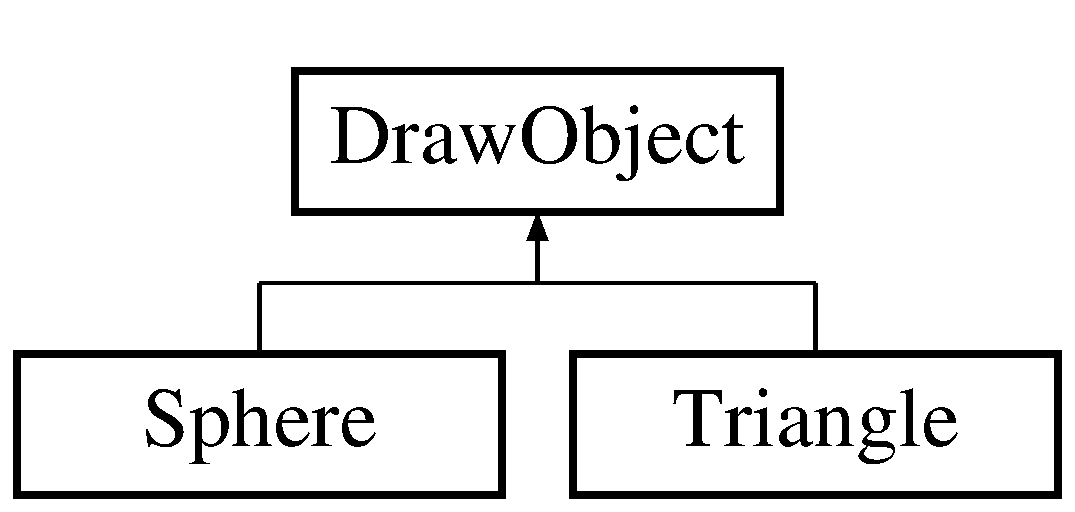
\includegraphics[height=2.000000cm]{class_draw_object}
\end{center}
\end{figure}
\subsection*{Public Member Functions}
\begin{DoxyCompactItemize}
\item 
\mbox{\Hypertarget{class_draw_object_a5dadd2f2acaa0153d5a987ca0774f4d2}\label{class_draw_object_a5dadd2f2acaa0153d5a987ca0774f4d2}} 
{\bfseries Draw\+Object} (string \+\_\+name)
\item 
\mbox{\Hypertarget{class_draw_object_afc75633fde3afcbdcd8b8b9953826992}\label{class_draw_object_afc75633fde3afcbdcd8b8b9953826992}} 
\hyperlink{class_material_base}{Material\+Base} $\ast$ {\bfseries Get\+Material} ()
\item 
\mbox{\Hypertarget{class_draw_object_a00b5eb5fbda278a316839cd38153321d}\label{class_draw_object_a00b5eb5fbda278a316839cd38153321d}} 
virtual bool {\bfseries Find\+Intersection} (\hyperlink{class_ray}{Ray} \&ray, float \&t)
\item 
\mbox{\Hypertarget{class_draw_object_a6851df385d257d299f9d4044e35a72a4}\label{class_draw_object_a6851df385d257d299f9d4044e35a72a4}} 
virtual \hyperlink{class_vector3f}{Vector3f} {\bfseries get\+Normal} (\hyperlink{class_vertex}{Vertex} hit)
\item 
\mbox{\Hypertarget{class_draw_object_a64a6ac1c3b730ad99244e9de160718a3}\label{class_draw_object_a64a6ac1c3b730ad99244e9de160718a3}} 
string {\bfseries Get\+Name} ()
\end{DoxyCompactItemize}
\subsection*{Static Public Attributes}
\begin{DoxyCompactItemize}
\item 
\mbox{\Hypertarget{class_draw_object_acf2061f9ae139591b6bee389945351bc}\label{class_draw_object_acf2061f9ae139591b6bee389945351bc}} 
static int {\bfseries number} = 0
\end{DoxyCompactItemize}


The documentation for this class was generated from the following file\+:\begin{DoxyCompactItemize}
\item 
sgl/sgl.\+cpp\end{DoxyCompactItemize}

\hypertarget{class_edge}{}\section{Edge Class Reference}
\label{class_edge}\index{Edge@{Edge}}
\subsection*{Public Member Functions}
\begin{DoxyCompactItemize}
\item 
\mbox{\Hypertarget{class_edge_a6ea465e0bd07ab5428ce26225bcb811e}\label{class_edge_a6ea465e0bd07ab5428ce26225bcb811e}} 
{\bfseries Edge} (float x1, float y1, float z1, float x2, float y2, float z2)
\item 
\mbox{\Hypertarget{class_edge_aa1c8cdcbd41e3b3b421df172e2aea77b}\label{class_edge_aa1c8cdcbd41e3b3b421df172e2aea77b}} 
float {\bfseries Get\+PositionX} ()
\item 
\mbox{\Hypertarget{class_edge_ae124ff527b00c86a16e49d992ce4fa0d}\label{class_edge_ae124ff527b00c86a16e49d992ce4fa0d}} 
float {\bfseries Get\+PositionY} ()
\item 
\mbox{\Hypertarget{class_edge_aeca4a489a032172e250a714b8c291c9e}\label{class_edge_aeca4a489a032172e250a714b8c291c9e}} 
float {\bfseries Get\+PositionZ} ()
\item 
\mbox{\Hypertarget{class_edge_aa8a5ad1d4b8575fdff96147e6f44c355}\label{class_edge_aa8a5ad1d4b8575fdff96147e6f44c355}} 
int {\bfseries Get\+DeltaY} ()
\item 
\mbox{\Hypertarget{class_edge_a1d52557b1b2ad4f45aa87965de567794}\label{class_edge_a1d52557b1b2ad4f45aa87965de567794}} 
bool {\bfseries Next\+Row} ()
\end{DoxyCompactItemize}


The documentation for this class was generated from the following file\+:\begin{DoxyCompactItemize}
\item 
sgl/sgl.\+cpp\end{DoxyCompactItemize}

\hypertarget{structevent_comparator}{}\section{event\+Comparator Struct Reference}
\label{structevent_comparator}\index{event\+Comparator@{event\+Comparator}}
\subsection*{Public Member Functions}
\begin{DoxyCompactItemize}
\item 
bool \hyperlink{structevent_comparator_a89a5486e6d21a0cdca230fc9c25c7bff}{operator()} (const \hyperlink{classtriangle_event}{triangle\+Event} $\ast$a, const \hyperlink{classtriangle_event}{triangle\+Event} $\ast$b)
\end{DoxyCompactItemize}


\subsection{Detailed Description}
Event comparator 

\subsection{Member Function Documentation}
\mbox{\Hypertarget{structevent_comparator_a89a5486e6d21a0cdca230fc9c25c7bff}\label{structevent_comparator_a89a5486e6d21a0cdca230fc9c25c7bff}} 
\index{event\+Comparator@{event\+Comparator}!operator()@{operator()}}
\index{operator()@{operator()}!event\+Comparator@{event\+Comparator}}
\subsubsection{\texorpdfstring{operator()()}{operator()()}}
{\footnotesize\ttfamily bool event\+Comparator\+::operator() (\begin{DoxyParamCaption}\item[{const \hyperlink{classtriangle_event}{triangle\+Event} $\ast$}]{a,  }\item[{const \hyperlink{classtriangle_event}{triangle\+Event} $\ast$}]{b }\end{DoxyParamCaption})\hspace{0.3cm}{\ttfamily [inline]}}

Event comparator as described in source paper ( $<$\+\_\+E ) 

The documentation for this struct was generated from the following file\+:\begin{DoxyCompactItemize}
\item 
sgl/sgl.\+cpp\end{DoxyCompactItemize}

\hypertarget{class_image_structure}{}\section{Image\+Structure Class Reference}
\label{class_image_structure}\index{Image\+Structure@{Image\+Structure}}
\subsection*{Public Member Functions}
\begin{DoxyCompactItemize}
\item 
\mbox{\Hypertarget{class_image_structure_abacb592e440dae8a781fec79668c6b0d}\label{class_image_structure_abacb592e440dae8a781fec79668c6b0d}} 
{\bfseries Image\+Structure} (int \+\_\+id, int \+\_\+width, int \+\_\+height)
\item 
\mbox{\Hypertarget{class_image_structure_a41206114ffee12e439bc5bac8a46ac1d}\label{class_image_structure_a41206114ffee12e439bc5bac8a46ac1d}} 
int {\bfseries Get\+Context\+ID} ()
\item 
\mbox{\Hypertarget{class_image_structure_a2245ecfc9d8cefdd5b45ccb2fc72580d}\label{class_image_structure_a2245ecfc9d8cefdd5b45ccb2fc72580d}} 
int {\bfseries Get\+Width} ()
\item 
\mbox{\Hypertarget{class_image_structure_a80da2e964cec395d6dc79be8a369e525}\label{class_image_structure_a80da2e964cec395d6dc79be8a369e525}} 
int {\bfseries Get\+Height} ()
\item 
\mbox{\Hypertarget{class_image_structure_a6d49c43c4dd8b6a6c632868239294371}\label{class_image_structure_a6d49c43c4dd8b6a6c632868239294371}} 
int {\bfseries Get\+Canvas\+Size} ()
\item 
\mbox{\Hypertarget{class_image_structure_a50a60a7b1d004850ec2481244bacaa1e}\label{class_image_structure_a50a60a7b1d004850ec2481244bacaa1e}} 
float $\ast$ {\bfseries Get\+Color\+Buffer} ()
\item 
\mbox{\Hypertarget{class_image_structure_aee62aa0f5fc1407652c9421b324b09b7}\label{class_image_structure_aee62aa0f5fc1407652c9421b324b09b7}} 
float $\ast$ {\bfseries Get\+Z\+Buffer} ()
\item 
\mbox{\Hypertarget{class_image_structure_ab40631d101553ff8b9110f36f5e60956}\label{class_image_structure_ab40631d101553ff8b9110f36f5e60956}} 
vector$<$ \hyperlink{class_vertex}{Vertex} $\ast$ $>$ $\ast$ {\bfseries Get\+Vertex\+Buffer} ()
\item 
\mbox{\Hypertarget{class_image_structure_a19d296f05d2b1db0c585dcb4aefb9577}\label{class_image_structure_a19d296f05d2b1db0c585dcb4aefb9577}} 
void {\bfseries Add\+Vertex} (float \+\_\+x, float \+\_\+y, float \+\_\+z=0, float \+\_\+w=1)
\item 
\mbox{\Hypertarget{class_image_structure_a27a8722b57e2c71ee56bea1c357c4624}\label{class_image_structure_a27a8722b57e2c71ee56bea1c357c4624}} 
void {\bfseries Clear\+Vertex\+Buffer} ()
\item 
\mbox{\Hypertarget{class_image_structure_a7a7359ab536e90c200ecac88802b15b5}\label{class_image_structure_a7a7359ab536e90c200ecac88802b15b5}} 
void {\bfseries Set\+Vertex\+Buffer} (vector$<$ \hyperlink{class_vertex}{Vertex} $\ast$$>$ $\ast$new\+\_\+vertex\+\_\+buffer)
\end{DoxyCompactItemize}


The documentation for this class was generated from the following file\+:\begin{DoxyCompactItemize}
\item 
sgl/sgl.\+cpp\end{DoxyCompactItemize}

\hypertarget{class_k_d___tree}{}\section{K\+D\+\_\+\+Tree Class Reference}
\label{class_k_d___tree}\index{K\+D\+\_\+\+Tree@{K\+D\+\_\+\+Tree}}


The documentation for this class was generated from the following file\+:\begin{DoxyCompactItemize}
\item 
sgl/sgl.\+cpp\end{DoxyCompactItemize}

\hypertarget{structkd_node}{}\section{kd\+Node Struct Reference}
\label{structkd_node}\index{kd\+Node@{kd\+Node}}
\subsection*{Public Attributes}
\begin{DoxyCompactItemize}
\item 
\mbox{\Hypertarget{structkd_node_a144866f55d774d1471f8f557ae17b001}\label{structkd_node_a144866f55d774d1471f8f557ae17b001}} 
\hyperlink{structkd_node}{kd\+Node} $\ast$ {\bfseries left} = N\+U\+LL
\item 
\mbox{\Hypertarget{structkd_node_a73f12ec56a1be783663f1f548d792674}\label{structkd_node_a73f12ec56a1be783663f1f548d792674}} 
\hyperlink{structkd_node}{kd\+Node} $\ast$ {\bfseries right} = N\+U\+LL
\item 
\mbox{\Hypertarget{structkd_node_addf0bbf5ea5bb36f77949d96e32046b8}\label{structkd_node_addf0bbf5ea5bb36f77949d96e32046b8}} 
\hyperlink{classsplit_plane}{split\+Plane} $\ast$ {\bfseries p} = N\+U\+LL
\item 
\mbox{\Hypertarget{structkd_node_afb1ac2fdc9cd3eb52d849855bedac531}\label{structkd_node_afb1ac2fdc9cd3eb52d849855bedac531}} 
bool {\bfseries N\+\_\+\+P\+\_\+left}
\end{DoxyCompactItemize}


\subsection{Detailed Description}
Structure representing one node in the kd-\/tree 

The documentation for this struct was generated from the following file\+:\begin{DoxyCompactItemize}
\item 
sgl/sgl.\+cpp\end{DoxyCompactItemize}

\hypertarget{class_material}{}\section{Material Class Reference}
\label{class_material}\index{Material@{Material}}
Inheritance diagram for Material\+:\begin{figure}[H]
\begin{center}
\leavevmode
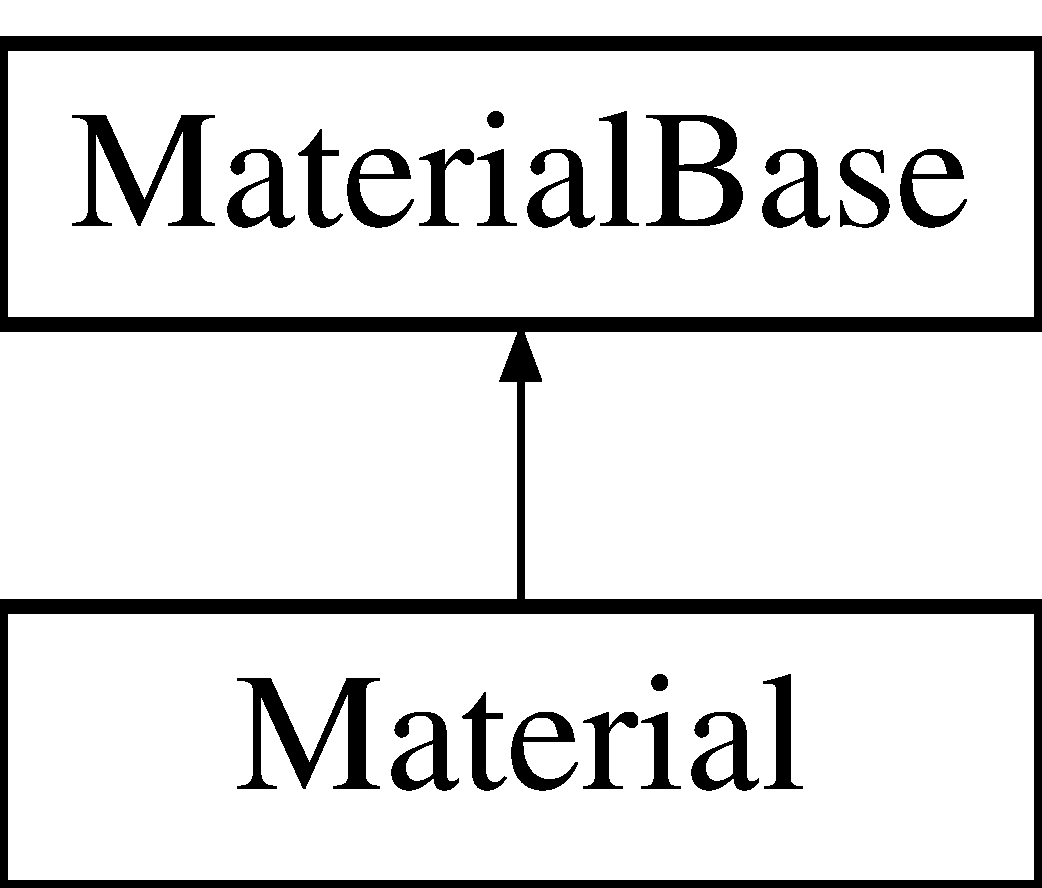
\includegraphics[height=2.000000cm]{class_material}
\end{center}
\end{figure}
\subsection*{Public Member Functions}
\begin{DoxyCompactItemize}
\item 
\mbox{\Hypertarget{class_material_a957af887ea4d0aaaa89f3319566e7af5}\label{class_material_a957af887ea4d0aaaa89f3319566e7af5}} 
{\bfseries Material} (float \+\_\+r, float \+\_\+g, float \+\_\+b, float \+\_\+kd, float \+\_\+ks, float \+\_\+shine, float \+\_\+T, float \+\_\+ior)
\item 
\mbox{\Hypertarget{class_material_ada6fe0016d0d41d8b63e7cad2889a092}\label{class_material_ada6fe0016d0d41d8b63e7cad2889a092}} 
\hyperlink{class_vector3f}{Vector3f} {\bfseries Get\+Diffuse} ()
\item 
\mbox{\Hypertarget{class_material_a23fa17b658a06e37945da193c90dcdec}\label{class_material_a23fa17b658a06e37945da193c90dcdec}} 
\hyperlink{class_vector3f}{Vector3f} {\bfseries Get\+Specular} ()
\item 
\mbox{\Hypertarget{class_material_a7362556d533530d59908cbd7ec0a799e}\label{class_material_a7362556d533530d59908cbd7ec0a799e}} 
float {\bfseries get\+Shine} ()
\item 
\mbox{\Hypertarget{class_material_a35f77eb9c342cc18cb649a9bccb8a86a}\label{class_material_a35f77eb9c342cc18cb649a9bccb8a86a}} 
float {\bfseries getT} ()
\item 
\mbox{\Hypertarget{class_material_a665dc0bbab498a7930b35fa1a6467830}\label{class_material_a665dc0bbab498a7930b35fa1a6467830}} 
float {\bfseries get\+Ior} ()
\item 
\mbox{\Hypertarget{class_material_ae456e321277b0b3ca7167e217f3cc3cd}\label{class_material_ae456e321277b0b3ca7167e217f3cc3cd}} 
\hyperlink{class_material}{Material} $\ast$ {\bfseries Deep\+Copy} ()
\end{DoxyCompactItemize}


The documentation for this class was generated from the following file\+:\begin{DoxyCompactItemize}
\item 
sgl/sgl.\+cpp\end{DoxyCompactItemize}

\hypertarget{class_material_base}{}\section{Material\+Base Class Reference}
\label{class_material_base}\index{Material\+Base@{Material\+Base}}
Inheritance diagram for Material\+Base\+:\begin{figure}[H]
\begin{center}
\leavevmode
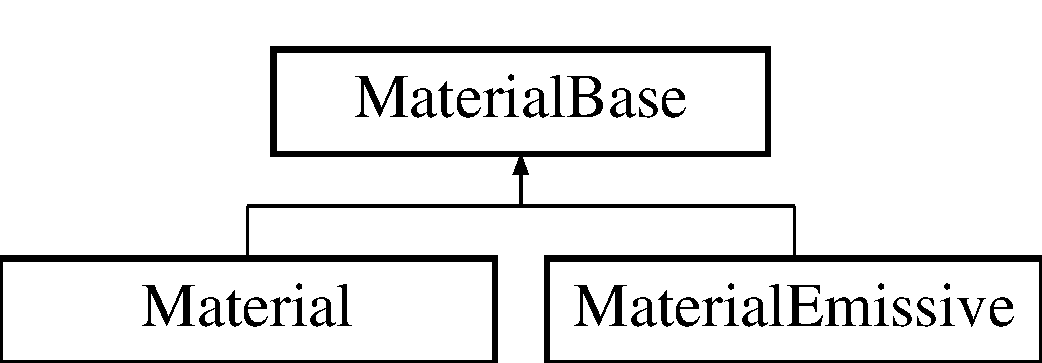
\includegraphics[height=2.000000cm]{class_material_base}
\end{center}
\end{figure}
\subsection*{Public Member Functions}
\begin{DoxyCompactItemize}
\item 
\mbox{\Hypertarget{class_material_base_a671519f0b0f36693096d8bec28ed49d8}\label{class_material_base_a671519f0b0f36693096d8bec28ed49d8}} 
{\bfseries Material\+Base} (bool emissive)
\item 
\mbox{\Hypertarget{class_material_base_a849fa0f00856923bc9585560fc7cc2c7}\label{class_material_base_a849fa0f00856923bc9585560fc7cc2c7}} 
virtual \hyperlink{class_material_base}{Material\+Base} $\ast$ {\bfseries Deep\+Copy} ()
\item 
\mbox{\Hypertarget{class_material_base_aacb0919ed97bec129b4d8c04bc23480e}\label{class_material_base_aacb0919ed97bec129b4d8c04bc23480e}} 
bool {\bfseries Emissive} ()
\end{DoxyCompactItemize}


The documentation for this class was generated from the following file\+:\begin{DoxyCompactItemize}
\item 
sgl/sgl.\+cpp\end{DoxyCompactItemize}

\hypertarget{class_material_emissive}{}\section{Material\+Emissive Class Reference}
\label{class_material_emissive}\index{Material\+Emissive@{Material\+Emissive}}
Inheritance diagram for Material\+Emissive\+:\begin{figure}[H]
\begin{center}
\leavevmode
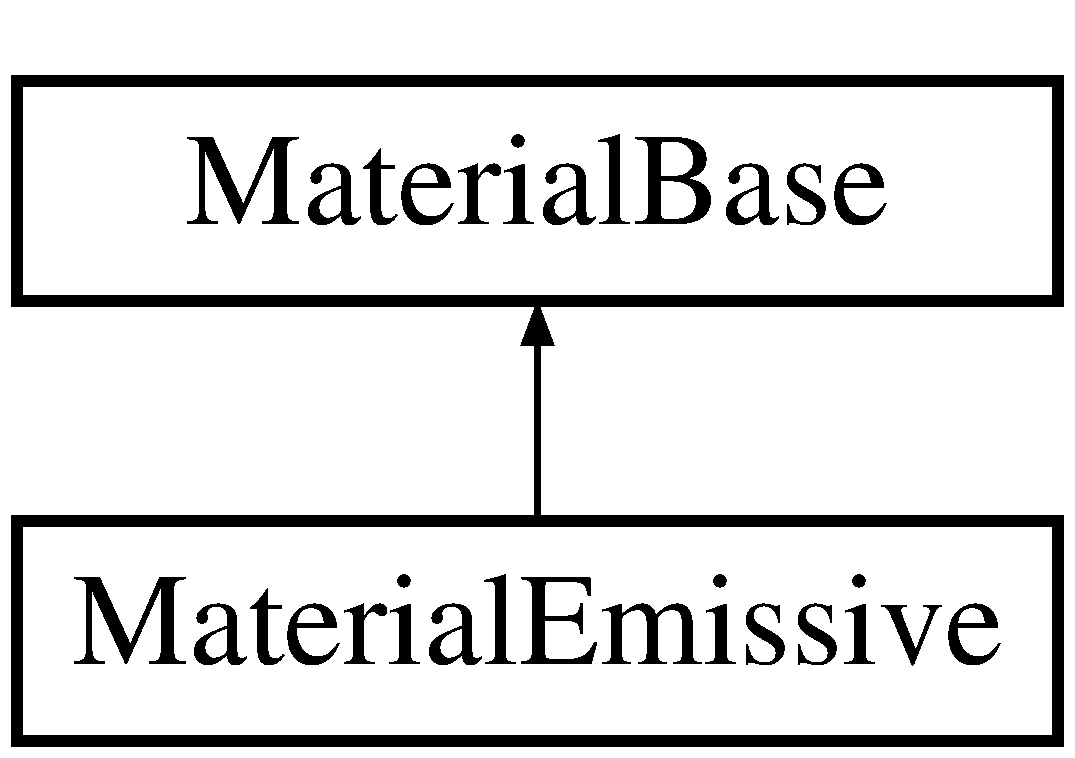
\includegraphics[height=2.000000cm]{class_material_emissive}
\end{center}
\end{figure}
\subsection*{Public Member Functions}
\begin{DoxyCompactItemize}
\item 
\mbox{\Hypertarget{class_material_emissive_aa269b64e4ea77d39af1bdeb65776246d}\label{class_material_emissive_aa269b64e4ea77d39af1bdeb65776246d}} 
{\bfseries Material\+Emissive} (float \+\_\+r, float \+\_\+g, float \+\_\+b, float \+\_\+c0, float \+\_\+c1, float \+\_\+c2)
\item 
\mbox{\Hypertarget{class_material_emissive_ac9290f5c0c1eb3c6e0931520018b08d5}\label{class_material_emissive_ac9290f5c0c1eb3c6e0931520018b08d5}} 
\hyperlink{class_vector3f}{Vector3f} {\bfseries Get\+Intensity} ()
\item 
\mbox{\Hypertarget{class_material_emissive_aeb4a407be901bc2d2f465d5cc1df9baf}\label{class_material_emissive_aeb4a407be901bc2d2f465d5cc1df9baf}} 
\hyperlink{class_vector3f}{Vector3f} {\bfseries Get\+Attentuation\+Cons} ()
\item 
\mbox{\Hypertarget{class_material_emissive_ae53e01766e3942ceb4a62bdc91309fb3}\label{class_material_emissive_ae53e01766e3942ceb4a62bdc91309fb3}} 
\hyperlink{class_material_emissive}{Material\+Emissive} $\ast$ {\bfseries Deep\+Copy} ()
\end{DoxyCompactItemize}


The documentation for this class was generated from the following file\+:\begin{DoxyCompactItemize}
\item 
sgl/sgl.\+cpp\end{DoxyCompactItemize}

\hypertarget{structplane_solution}{}\section{plane\+Solution Struct Reference}
\label{structplane_solution}\index{plane\+Solution@{plane\+Solution}}
\subsection*{Public Attributes}
\begin{DoxyCompactItemize}
\item 
\mbox{\Hypertarget{structplane_solution_ad6c9c6f73f2d473915001d266fbc8d5d}\label{structplane_solution_ad6c9c6f73f2d473915001d266fbc8d5d}} 
\hyperlink{classsplit_plane}{split\+Plane} $\ast$ {\bfseries plane}
\item 
\mbox{\Hypertarget{structplane_solution_a8aae0a96589badef74ee4aeed61e9b74}\label{structplane_solution_a8aae0a96589badef74ee4aeed61e9b74}} 
float {\bfseries cost}
\end{DoxyCompactItemize}


\subsection{Detailed Description}
Structure containing a split plane candidate, its cost and whether the triangles in the plane should be moved to left or right 

The documentation for this struct was generated from the following file\+:\begin{DoxyCompactItemize}
\item 
sgl/sgl.\+cpp\end{DoxyCompactItemize}

\hypertarget{class_point_light}{}\section{Point\+Light Class Reference}
\label{class_point_light}\index{Point\+Light@{Point\+Light}}
\subsection*{Public Member Functions}
\begin{DoxyCompactItemize}
\item 
\mbox{\Hypertarget{class_point_light_a62f5a67c145c369d4dc3b6b74f7b4905}\label{class_point_light_a62f5a67c145c369d4dc3b6b74f7b4905}} 
{\bfseries Point\+Light} (float x, float y, float z, float \+\_\+r, float \+\_\+g, float \+\_\+b)
\item 
\mbox{\Hypertarget{class_point_light_a3a312a3daa19fb015586c3fdc57b7b5f}\label{class_point_light_a3a312a3daa19fb015586c3fdc57b7b5f}} 
\hyperlink{class_vertex}{Vertex} $\ast$ {\bfseries Get\+Position} ()
\item 
\mbox{\Hypertarget{class_point_light_af030c584752d3c91299e32b25346a30e}\label{class_point_light_af030c584752d3c91299e32b25346a30e}} 
\hyperlink{class_vector3f}{Vector3f} $\ast$ {\bfseries Get\+Intensity} ()
\end{DoxyCompactItemize}


The documentation for this class was generated from the following file\+:\begin{DoxyCompactItemize}
\item 
sgl/sgl.\+cpp\end{DoxyCompactItemize}

\hypertarget{class_ray}{}\section{Ray Class Reference}
\label{class_ray}\index{Ray@{Ray}}
\subsection*{Public Member Functions}
\begin{DoxyCompactItemize}
\item 
\mbox{\Hypertarget{class_ray_a156a9e2a3055e58a52622077a5e36f3c}\label{class_ray_a156a9e2a3055e58a52622077a5e36f3c}} 
{\bfseries Ray} (float x\+\_\+start, float y\+\_\+start, float z\+\_\+start, float x\+\_\+end, float y\+\_\+end, float z\+\_\+end)
\end{DoxyCompactItemize}
\subsection*{Public Attributes}
\begin{DoxyCompactItemize}
\item 
\mbox{\Hypertarget{class_ray_a948bb948f30f54627d9b316433cc5d69}\label{class_ray_a948bb948f30f54627d9b316433cc5d69}} 
\hyperlink{class_vertex}{Vertex} $\ast$ {\bfseries origin}
\item 
\mbox{\Hypertarget{class_ray_a6b0d90f41edce755b0cedab9300c4535}\label{class_ray_a6b0d90f41edce755b0cedab9300c4535}} 
\hyperlink{class_vertex}{Vertex} $\ast$ {\bfseries direction}
\end{DoxyCompactItemize}


The documentation for this class was generated from the following file\+:\begin{DoxyCompactItemize}
\item 
sgl/sgl.\+cpp\end{DoxyCompactItemize}

\hypertarget{class_scene_structure}{}\section{Scene\+Structure Class Reference}
\label{class_scene_structure}\index{Scene\+Structure@{Scene\+Structure}}
\subsection*{Public Member Functions}
\begin{DoxyCompactItemize}
\item 
\mbox{\Hypertarget{class_scene_structure_ad07922a4fce33965a58d734b0012cfae}\label{class_scene_structure_ad07922a4fce33965a58d734b0012cfae}} 
void {\bfseries Add\+Primitive} (float x, float y, float z, float \+\_\+radius)
\item 
\mbox{\Hypertarget{class_scene_structure_aa2e30b5b1a0a2681de75734ad7a3f1b7}\label{class_scene_structure_aa2e30b5b1a0a2681de75734ad7a3f1b7}} 
void {\bfseries Add\+Primitive} (sgl\+E\+Element\+Type \+\_\+object\+\_\+type, vector$<$ \hyperlink{class_vertex}{Vertex} $\ast$$>$ $\ast$\+\_\+vertices, bool emissive)
\item 
\mbox{\Hypertarget{class_scene_structure_aa7c8ce8bb44a06f0f02801abde3eecfc}\label{class_scene_structure_aa7c8ce8bb44a06f0f02801abde3eecfc}} 
void {\bfseries Add\+Light} (float x, float y, float z, float r, float g, float b)
\item 
\mbox{\Hypertarget{class_scene_structure_a8a98d6e4d0f7f33297e6c6f173c2cece}\label{class_scene_structure_a8a98d6e4d0f7f33297e6c6f173c2cece}} 
\hyperlink{class_draw_object}{Draw\+Object} $\ast$ {\bfseries Find\+Intersection} (\hyperlink{class_ray}{Ray} \&ray, float \&dist)
\item 
\mbox{\Hypertarget{class_scene_structure_a072429ad6386e5f8879727b0f0734a39}\label{class_scene_structure_a072429ad6386e5f8879727b0f0734a39}} 
\hyperlink{class_draw_object}{Draw\+Object} $\ast$ {\bfseries Find\+Shadow\+Intersection} (\hyperlink{class_ray}{Ray} \&ray, float \&dist, \hyperlink{class_draw_object}{Draw\+Object} $\ast$obj)
\item 
\mbox{\Hypertarget{class_scene_structure_ab1119698dc99ceb6b73c5fbe6efc5afe}\label{class_scene_structure_ab1119698dc99ceb6b73c5fbe6efc5afe}} 
\hyperlink{class_vector3f}{Vector3f} {\bfseries Illuminate} (\hyperlink{class_draw_object}{Draw\+Object} $\ast$object, \hyperlink{class_ray}{Ray} \&ray, float distance, int level)
\end{DoxyCompactItemize}


The documentation for this class was generated from the following file\+:\begin{DoxyCompactItemize}
\item 
sgl/sgl.\+cpp\end{DoxyCompactItemize}

\hypertarget{class_sphere}{}\section{Sphere Class Reference}
\label{class_sphere}\index{Sphere@{Sphere}}
Inheritance diagram for Sphere\+:\begin{figure}[H]
\begin{center}
\leavevmode
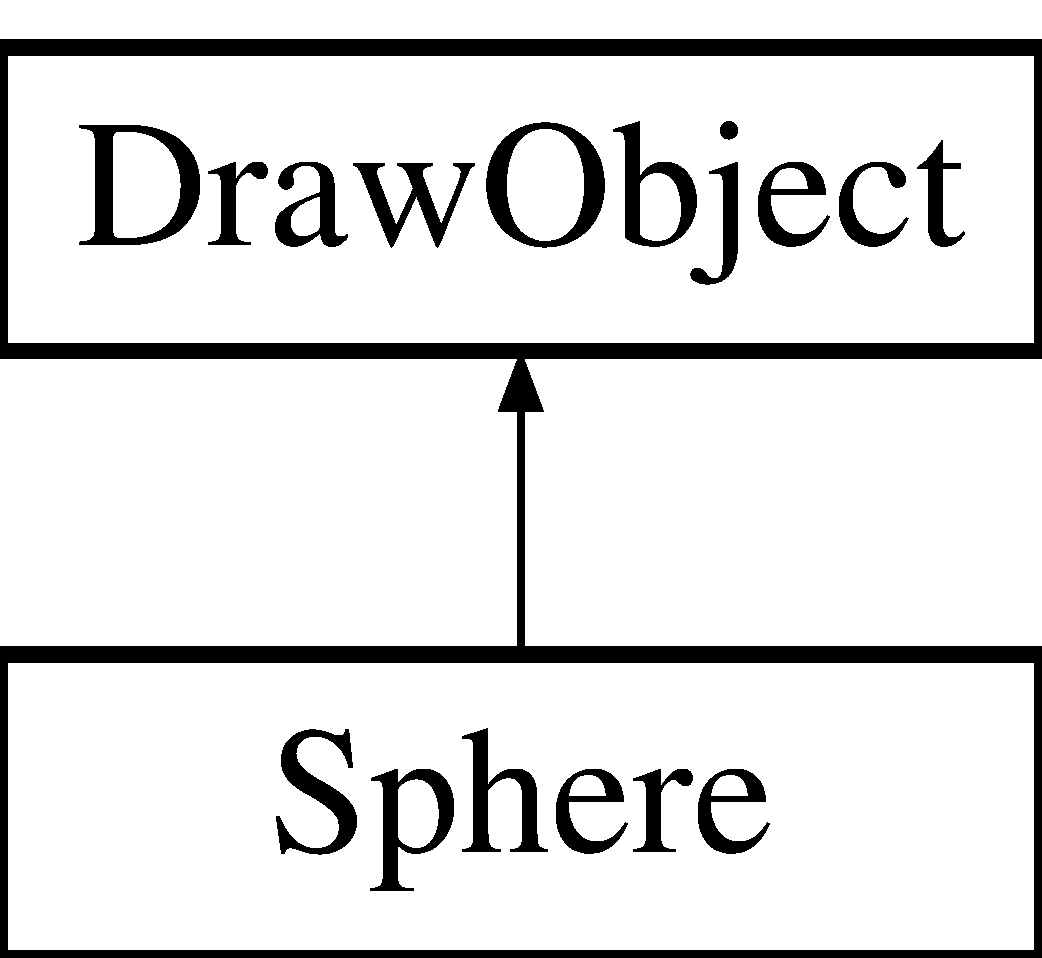
\includegraphics[height=2.000000cm]{class_sphere}
\end{center}
\end{figure}
\subsection*{Public Member Functions}
\begin{DoxyCompactItemize}
\item 
\mbox{\Hypertarget{class_sphere_a9a4226026f582a564c5d02939bb0f232}\label{class_sphere_a9a4226026f582a564c5d02939bb0f232}} 
{\bfseries Sphere} (float x, float y, float z, float \+\_\+radius)
\item 
\mbox{\Hypertarget{class_sphere_acbad5180e6fd66b3f95d29cfa1139458}\label{class_sphere_acbad5180e6fd66b3f95d29cfa1139458}} 
virtual bool {\bfseries Find\+Intersection} (\hyperlink{class_ray}{Ray} \&ray, float \&distance)
\item 
\mbox{\Hypertarget{class_sphere_a89d2bfb75666f496514bd35c2e23a1ce}\label{class_sphere_a89d2bfb75666f496514bd35c2e23a1ce}} 
virtual \hyperlink{class_vector3f}{Vector3f} {\bfseries get\+Normal} (\hyperlink{class_vertex}{Vertex} hit)
\end{DoxyCompactItemize}
\subsection*{Additional Inherited Members}


The documentation for this class was generated from the following file\+:\begin{DoxyCompactItemize}
\item 
sgl/sgl.\+cpp\end{DoxyCompactItemize}

\hypertarget{classsplit_plane}{}\section{split\+Plane Class Reference}
\label{classsplit_plane}\index{split\+Plane@{split\+Plane}}
\subsection*{Public Member Functions}
\begin{DoxyCompactItemize}
\item 
\mbox{\Hypertarget{classsplit_plane_a816412b8c1b3f5b871fff0d8f372f287}\label{classsplit_plane_a816412b8c1b3f5b871fff0d8f372f287}} 
{\bfseries split\+Plane} (float position, int dimension, bool left)
\end{DoxyCompactItemize}
\subsection*{Public Attributes}
\begin{DoxyCompactItemize}
\item 
\mbox{\Hypertarget{classsplit_plane_ad814131a437d5145b440a7589d37c10b}\label{classsplit_plane_ad814131a437d5145b440a7589d37c10b}} 
float {\bfseries position}
\item 
\mbox{\Hypertarget{classsplit_plane_a18948f11f0776d35adf861b198554380}\label{classsplit_plane_a18948f11f0776d35adf861b198554380}} 
int {\bfseries dimension}
\item 
\mbox{\Hypertarget{classsplit_plane_aa261e4e8ae1c7e16efa1069c8eb3aaca}\label{classsplit_plane_aa261e4e8ae1c7e16efa1069c8eb3aaca}} 
bool {\bfseries left}
\end{DoxyCompactItemize}


\subsection{Detailed Description}
Class used for split plane representation 

The documentation for this class was generated from the following file\+:\begin{DoxyCompactItemize}
\item 
sgl/sgl.\+cpp\end{DoxyCompactItemize}

\hypertarget{class_transformation_stack}{}\section{Transformation\+Stack Class Reference}
\label{class_transformation_stack}\index{Transformation\+Stack@{Transformation\+Stack}}
\subsection*{Public Member Functions}
\begin{DoxyCompactItemize}
\item 
\mbox{\Hypertarget{class_transformation_stack_a30b49bc49cd2b57494c1b25f60e093f7}\label{class_transformation_stack_a30b49bc49cd2b57494c1b25f60e093f7}} 
float $\ast$ {\bfseries Get\+Current} ()
\item 
\mbox{\Hypertarget{class_transformation_stack_ae7073bc34c342e84f34012bfb90e0046}\label{class_transformation_stack_ae7073bc34c342e84f34012bfb90e0046}} 
void {\bfseries set\+Current} (float $\ast$matrix)
\item 
\mbox{\Hypertarget{class_transformation_stack_a1c4966cc4a17a9815bda6cbe659bd48b}\label{class_transformation_stack_a1c4966cc4a17a9815bda6cbe659bd48b}} 
void {\bfseries pop} ()
\item 
\mbox{\Hypertarget{class_transformation_stack_a0c1b1e028385d0e5cfc8fa7892637d98}\label{class_transformation_stack_a0c1b1e028385d0e5cfc8fa7892637d98}} 
void {\bfseries push} ()
\item 
\mbox{\Hypertarget{class_transformation_stack_ad9e01004403853199f72df5ddf067360}\label{class_transformation_stack_ad9e01004403853199f72df5ddf067360}} 
bool {\bfseries check\+Empty\+Stack} ()
\end{DoxyCompactItemize}


The documentation for this class was generated from the following file\+:\begin{DoxyCompactItemize}
\item 
sgl/sgl.\+cpp\end{DoxyCompactItemize}

\hypertarget{class_triangle}{}\section{Triangle Class Reference}
\label{class_triangle}\index{Triangle@{Triangle}}
Inheritance diagram for Triangle\+:\begin{figure}[H]
\begin{center}
\leavevmode
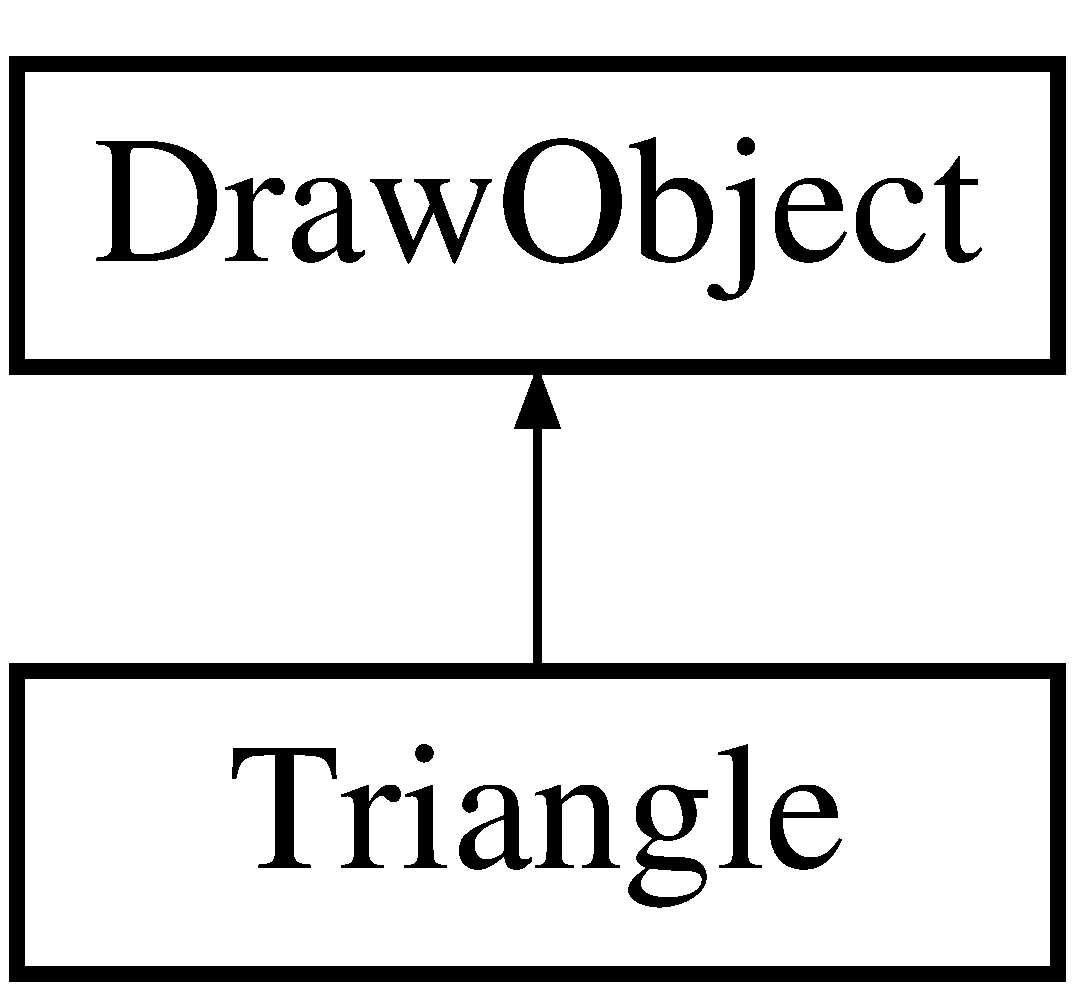
\includegraphics[height=2.000000cm]{class_triangle}
\end{center}
\end{figure}
\subsection*{Public Member Functions}
\begin{DoxyCompactItemize}
\item 
\mbox{\Hypertarget{class_triangle_aea5e936b8cb88b19c5cf6e9704bc13db}\label{class_triangle_aea5e936b8cb88b19c5cf6e9704bc13db}} 
{\bfseries Triangle} (sgl\+E\+Element\+Type \+\_\+object\+\_\+type, vector$<$ \hyperlink{class_vertex}{Vertex} $\ast$$>$ $\ast$\+\_\+vertices)
\item 
\mbox{\Hypertarget{class_triangle_a5928933b2095b43375a38f48ec265c32}\label{class_triangle_a5928933b2095b43375a38f48ec265c32}} 
virtual bool {\bfseries Find\+Intersection} (\hyperlink{class_ray}{Ray} \&ray, float \&t\+Hit)
\item 
\mbox{\Hypertarget{class_triangle_aa2ba0470a4524e65335e1729bb5df109}\label{class_triangle_aa2ba0470a4524e65335e1729bb5df109}} 
virtual \hyperlink{class_vector3f}{Vector3f} {\bfseries get\+Normal} (\hyperlink{class_vertex}{Vertex} hit)
\item 
\mbox{\Hypertarget{class_triangle_a120fc129e68a5b04f9ad8a67a383f9c1}\label{class_triangle_a120fc129e68a5b04f9ad8a67a383f9c1}} 
\hyperlink{class_vertex}{Vertex} {\bfseries random\+Sample} ()
\item 
\mbox{\Hypertarget{class_triangle_adb5bf3b29239d6758ad301627f2bebbc}\label{class_triangle_adb5bf3b29239d6758ad301627f2bebbc}} 
float {\bfseries area\+Size} ()
\item 
\mbox{\Hypertarget{class_triangle_a38afc42ec5be95a7320366b170cca749}\label{class_triangle_a38afc42ec5be95a7320366b170cca749}} 
vector$<$ \hyperlink{class_vertex}{Vertex} $\ast$ $>$ $\ast$ {\bfseries get\+Vertices} ()
\end{DoxyCompactItemize}
\subsection*{Additional Inherited Members}


The documentation for this class was generated from the following file\+:\begin{DoxyCompactItemize}
\item 
sgl/sgl.\+cpp\end{DoxyCompactItemize}

\hypertarget{classtriangle_event}{}\section{triangle\+Event Class Reference}
\label{classtriangle_event}\index{triangle\+Event@{triangle\+Event}}
\subsection*{Public Attributes}
\begin{DoxyCompactItemize}
\item 
int \hyperlink{classtriangle_event_a0e413f5b305dbe0c27b8e0d38a81b7ad}{dimension}
\item 
float \hyperlink{classtriangle_event_a201ec4ed38941f5e592258e8ded88ef2}{coordinate}
\item 
int \hyperlink{classtriangle_event_a78388041677d097127500270b580826c}{type}
\item 
int \hyperlink{classtriangle_event_ae36abd7d179b513bed4caff1a85d9730}{triangle\+ID}
\end{DoxyCompactItemize}


\subsection{Detailed Description}
Class used for representation of a triangle event 

\subsection{Member Data Documentation}
\mbox{\Hypertarget{classtriangle_event_a201ec4ed38941f5e592258e8ded88ef2}\label{classtriangle_event_a201ec4ed38941f5e592258e8ded88ef2}} 
\index{triangle\+Event@{triangle\+Event}!coordinate@{coordinate}}
\index{coordinate@{coordinate}!triangle\+Event@{triangle\+Event}}
\subsubsection{\texorpdfstring{coordinate}{coordinate}}
{\footnotesize\ttfamily float triangle\+Event\+::coordinate}

position of the event in dimension specified by the above variable dimension \mbox{\Hypertarget{classtriangle_event_a0e413f5b305dbe0c27b8e0d38a81b7ad}\label{classtriangle_event_a0e413f5b305dbe0c27b8e0d38a81b7ad}} 
\index{triangle\+Event@{triangle\+Event}!dimension@{dimension}}
\index{dimension@{dimension}!triangle\+Event@{triangle\+Event}}
\subsubsection{\texorpdfstring{dimension}{dimension}}
{\footnotesize\ttfamily int triangle\+Event\+::dimension}

Dimension to which this events add a potential split candidate \mbox{\Hypertarget{classtriangle_event_ae36abd7d179b513bed4caff1a85d9730}\label{classtriangle_event_ae36abd7d179b513bed4caff1a85d9730}} 
\index{triangle\+Event@{triangle\+Event}!triangle\+ID@{triangle\+ID}}
\index{triangle\+ID@{triangle\+ID}!triangle\+Event@{triangle\+Event}}
\subsubsection{\texorpdfstring{triangle\+ID}{triangleID}}
{\footnotesize\ttfamily int triangle\+Event\+::triangle\+ID}

ID of corresponding triangle in the triangle vector (specific to it\textquotesingle{}s recursion level) \mbox{\Hypertarget{classtriangle_event_a78388041677d097127500270b580826c}\label{classtriangle_event_a78388041677d097127500270b580826c}} 
\index{triangle\+Event@{triangle\+Event}!type@{type}}
\index{type@{type}!triangle\+Event@{triangle\+Event}}
\subsubsection{\texorpdfstring{type}{type}}
{\footnotesize\ttfamily int triangle\+Event\+::type}

consistently with the Tau function, type == 0 if the events is an end event, 1 if it is a planar event and 2 if it is a start event 

The documentation for this class was generated from the following file\+:\begin{DoxyCompactItemize}
\item 
sgl/sgl.\+cpp\end{DoxyCompactItemize}

\hypertarget{class_vector3f}{}\section{Vector3f Class Reference}
\label{class_vector3f}\index{Vector3f@{Vector3f}}
\subsection*{Public Member Functions}
\begin{DoxyCompactItemize}
\item 
\mbox{\Hypertarget{class_vector3f_a44a7820fe5223bebb6ef902c3942a96a}\label{class_vector3f_a44a7820fe5223bebb6ef902c3942a96a}} 
{\bfseries Vector3f} (\hyperlink{class_vertex}{Vertex} $\ast$old)
\item 
\mbox{\Hypertarget{class_vector3f_ac2caf1fd41076826fe50b3a527ef90db}\label{class_vector3f_ac2caf1fd41076826fe50b3a527ef90db}} 
{\bfseries Vector3f} (float \+\_\+x, float \+\_\+y, float \+\_\+z)
\item 
\mbox{\Hypertarget{class_vector3f_ad2b60dc77ac826601b53dfbe00a10e8b}\label{class_vector3f_ad2b60dc77ac826601b53dfbe00a10e8b}} 
\hyperlink{class_vector3f}{Vector3f} {\bfseries operator-\/} (\hyperlink{class_vector3f}{Vector3f} v2)
\item 
\mbox{\Hypertarget{class_vector3f_a825c94e2a03cf1848f326090d870a48b}\label{class_vector3f_a825c94e2a03cf1848f326090d870a48b}} 
\hyperlink{class_vector3f}{Vector3f} {\bfseries operator-\/} (\hyperlink{class_vertex}{Vertex} $\ast$v2)
\item 
\mbox{\Hypertarget{class_vector3f_a8c508043e7a51811690aa0f7621d27ad}\label{class_vector3f_a8c508043e7a51811690aa0f7621d27ad}} 
\hyperlink{class_vector3f}{Vector3f} {\bfseries operator-\/} (\hyperlink{class_vertex}{Vertex} v2)
\item 
\mbox{\Hypertarget{class_vector3f_aac989fe2139af72f485aff7bd834f7ba}\label{class_vector3f_aac989fe2139af72f485aff7bd834f7ba}} 
\hyperlink{class_vector3f}{Vector3f} {\bfseries operator+} (\hyperlink{class_vertex}{Vertex} v2)
\item 
\mbox{\Hypertarget{class_vector3f_aefe47612044b40b40ae99bd1bdb6a6b7}\label{class_vector3f_aefe47612044b40b40ae99bd1bdb6a6b7}} 
\hyperlink{class_vector3f}{Vector3f} {\bfseries operator+} (\hyperlink{class_vector3f}{Vector3f} v2)
\item 
\mbox{\Hypertarget{class_vector3f_ad0b4d24609bb325fa4255f40c09d71d4}\label{class_vector3f_ad0b4d24609bb325fa4255f40c09d71d4}} 
\hyperlink{class_vector3f}{Vector3f} {\bfseries operator$\ast$} (float v)
\item 
\mbox{\Hypertarget{class_vector3f_a4a1505e87eb9d13a6aeded805aeb92bb}\label{class_vector3f_a4a1505e87eb9d13a6aeded805aeb92bb}} 
\hyperlink{class_vector3f}{Vector3f} {\bfseries operator$\ast$} (\hyperlink{class_vertex}{Vertex} v2)
\item 
\mbox{\Hypertarget{class_vector3f_a3affdcd47ad900f87e9ff310efd37a7e}\label{class_vector3f_a3affdcd47ad900f87e9ff310efd37a7e}} 
\hyperlink{class_vector3f}{Vector3f} {\bfseries operator$\ast$} (\hyperlink{class_vector3f}{Vector3f} v2)
\item 
\mbox{\Hypertarget{class_vector3f_a4ea1191fa08b53a058d6bd0994421bad}\label{class_vector3f_a4ea1191fa08b53a058d6bd0994421bad}} 
\hyperlink{class_vector3f}{Vector3f} {\bfseries operator/} (float v)
\item 
\mbox{\Hypertarget{class_vector3f_a0be10a85c33bb64628c4934b42cc16fd}\label{class_vector3f_a0be10a85c33bb64628c4934b42cc16fd}} 
void {\bfseries operator=} (\hyperlink{class_vertex}{Vertex} v2)
\item 
\mbox{\Hypertarget{class_vector3f_afd0805b398d4b20e84a7b00aed7782eb}\label{class_vector3f_afd0805b398d4b20e84a7b00aed7782eb}} 
void {\bfseries operator=} (\hyperlink{class_vector3f}{Vector3f} v2)
\item 
\mbox{\Hypertarget{class_vector3f_a7ae034cf6d017074dfe1fdac8e251671}\label{class_vector3f_a7ae034cf6d017074dfe1fdac8e251671}} 
void {\bfseries Normalize} ()
\end{DoxyCompactItemize}
\subsection*{Static Public Member Functions}
\begin{DoxyCompactItemize}
\item 
\mbox{\Hypertarget{class_vector3f_aae3f6360e241157bef0ba864a3d441bf}\label{class_vector3f_aae3f6360e241157bef0ba864a3d441bf}} 
static float {\bfseries Dot\+Product} (\hyperlink{class_vector3f}{Vector3f} \&v1, \hyperlink{class_vector3f}{Vector3f} \&v2)
\end{DoxyCompactItemize}
\subsection*{Public Attributes}
\begin{DoxyCompactItemize}
\item 
\mbox{\Hypertarget{class_vector3f_a4aca0751716b7099b397e8c63b16bfcf}\label{class_vector3f_a4aca0751716b7099b397e8c63b16bfcf}} 
float {\bfseries x}
\item 
\mbox{\Hypertarget{class_vector3f_a8a602e2ee75126feb520c2aa27e7eff5}\label{class_vector3f_a8a602e2ee75126feb520c2aa27e7eff5}} 
float {\bfseries y}
\item 
\mbox{\Hypertarget{class_vector3f_a470cff51eb6463672be518f5af4e26db}\label{class_vector3f_a470cff51eb6463672be518f5af4e26db}} 
float {\bfseries z}
\end{DoxyCompactItemize}


The documentation for this class was generated from the following file\+:\begin{DoxyCompactItemize}
\item 
sgl/sgl.\+cpp\end{DoxyCompactItemize}

\hypertarget{class_vertex}{}\section{Vertex Class Reference}
\label{class_vertex}\index{Vertex@{Vertex}}
\subsection*{Public Member Functions}
\begin{DoxyCompactItemize}
\item 
\mbox{\Hypertarget{class_vertex_af28074c8f359c2c815ef2f164bf6355b}\label{class_vertex_af28074c8f359c2c815ef2f164bf6355b}} 
{\bfseries Vertex} (float \+\_\+x, float \+\_\+y, float \+\_\+z, float \+\_\+w)
\item 
\mbox{\Hypertarget{class_vertex_aa78d4c3433559e6e50260240c49a3d03}\label{class_vertex_aa78d4c3433559e6e50260240c49a3d03}} 
float {\bfseries getX} ()
\item 
\mbox{\Hypertarget{class_vertex_a12facdc9f554fd718e449f2aa2eefeaf}\label{class_vertex_a12facdc9f554fd718e449f2aa2eefeaf}} 
float {\bfseries getY} ()
\item 
\mbox{\Hypertarget{class_vertex_a258fea59f7c07f4e8784fc90c6ac7cb3}\label{class_vertex_a258fea59f7c07f4e8784fc90c6ac7cb3}} 
float {\bfseries getZ} ()
\item 
\mbox{\Hypertarget{class_vertex_a6957f8fb928fb151b260efc8dfe10455}\label{class_vertex_a6957f8fb928fb151b260efc8dfe10455}} 
float {\bfseries getW} ()
\item 
\mbox{\Hypertarget{class_vertex_a5d5284346279af944480cce75013dfa7}\label{class_vertex_a5d5284346279af944480cce75013dfa7}} 
\hyperlink{class_vertex}{Vertex} {\bfseries normalize} ()
\item 
\mbox{\Hypertarget{class_vertex_af7e2b7c7b9cba4ff94f9bca7bc389e2e}\label{class_vertex_af7e2b7c7b9cba4ff94f9bca7bc389e2e}} 
void {\bfseries divide\+ByW} ()
\item 
\mbox{\Hypertarget{class_vertex_a16cdfc490098f9d1e59a134d842f7039}\label{class_vertex_a16cdfc490098f9d1e59a134d842f7039}} 
void {\bfseries normalize\+This} ()
\item 
\mbox{\Hypertarget{class_vertex_a287781f2ff321c0734662ff48008ad52}\label{class_vertex_a287781f2ff321c0734662ff48008ad52}} 
\hyperlink{class_vertex}{Vertex} {\bfseries operator-\/} (\hyperlink{class_vertex}{Vertex} v2)
\item 
\mbox{\Hypertarget{class_vertex_a9664c1135530ea8a00ba4df5fae13bf1}\label{class_vertex_a9664c1135530ea8a00ba4df5fae13bf1}} 
\hyperlink{class_vertex}{Vertex} {\bfseries operator+} (\hyperlink{class_vertex}{Vertex} v2)
\item 
\mbox{\Hypertarget{class_vertex_a7f9ab7e0df3e5c72faf8069379a88a89}\label{class_vertex_a7f9ab7e0df3e5c72faf8069379a88a89}} 
\hyperlink{class_vertex}{Vertex} {\bfseries operator$\ast$} (float v)
\end{DoxyCompactItemize}
\subsection*{Static Public Member Functions}
\begin{DoxyCompactItemize}
\item 
\mbox{\Hypertarget{class_vertex_a90c0b93ebbbaf3e686416d3c0efb3915}\label{class_vertex_a90c0b93ebbbaf3e686416d3c0efb3915}} 
static float {\bfseries Dot\+Product} (\hyperlink{class_vertex}{Vertex} \&v1, \hyperlink{class_vertex}{Vertex} v2)
\item 
\mbox{\Hypertarget{class_vertex_acf36b7b488e2b11975bc8d861685913b}\label{class_vertex_acf36b7b488e2b11975bc8d861685913b}} 
static float {\bfseries Distance} (\hyperlink{class_vertex}{Vertex} v1, \hyperlink{class_vertex}{Vertex} v2)
\end{DoxyCompactItemize}


The documentation for this class was generated from the following file\+:\begin{DoxyCompactItemize}
\item 
sgl/sgl.\+cpp\end{DoxyCompactItemize}

\hypertarget{class_voxel}{}\section{Voxel Class Reference}
\label{class_voxel}\index{Voxel@{Voxel}}
\subsection*{Public Member Functions}
\begin{DoxyCompactItemize}
\item 
\mbox{\Hypertarget{class_voxel_a75fa478cf4d24275622e9d954d2bf2c7}\label{class_voxel_a75fa478cf4d24275622e9d954d2bf2c7}} 
{\bfseries Voxel} (\hyperlink{class_vector3f}{Vector3f} \hyperlink{class_voxel_a92eee751b0eaf4d10e4b5aa8f4f749ef}{position}, float \hyperlink{class_voxel_a1e494958e8f6d557a0b9ef65fb445322}{dX}, float \hyperlink{class_voxel_ad7366d4015819afbebd6c5035d694efa}{dY}, float \hyperlink{class_voxel_a58964f88e01b0aed80e993e6aad25f24}{dZ})
\item 
\mbox{\Hypertarget{class_voxel_afc909b1392d8d211ec35e280eb4bb785}\label{class_voxel_afc909b1392d8d211ec35e280eb4bb785}} 
void {\bfseries set\+Position} (\hyperlink{class_vector3f}{Vector3f} \hyperlink{class_voxel_a92eee751b0eaf4d10e4b5aa8f4f749ef}{position})
\item 
pair$<$ \hyperlink{class_voxel}{Voxel} $\ast$, \hyperlink{class_voxel}{Voxel} $\ast$ $>$ \hyperlink{class_voxel_ac205abe6c14926c43c021422eef6a996}{split\+By\+Plane} (\hyperlink{classsplit_plane}{split\+Plane} $\ast$p)
\end{DoxyCompactItemize}
\subsection*{Public Attributes}
\begin{DoxyCompactItemize}
\item 
\hyperlink{class_vector3f}{Vector3f} \hyperlink{class_voxel_a92eee751b0eaf4d10e4b5aa8f4f749ef}{position}
\item 
float \hyperlink{class_voxel_a1e494958e8f6d557a0b9ef65fb445322}{dX}
\item 
float \hyperlink{class_voxel_ad7366d4015819afbebd6c5035d694efa}{dY}
\item 
float \hyperlink{class_voxel_a58964f88e01b0aed80e993e6aad25f24}{dZ}
\end{DoxyCompactItemize}


\subsection{Detailed Description}
Class used for voxel representation 

\subsection{Member Function Documentation}
\mbox{\Hypertarget{class_voxel_ac205abe6c14926c43c021422eef6a996}\label{class_voxel_ac205abe6c14926c43c021422eef6a996}} 
\index{Voxel@{Voxel}!split\+By\+Plane@{split\+By\+Plane}}
\index{split\+By\+Plane@{split\+By\+Plane}!Voxel@{Voxel}}
\subsubsection{\texorpdfstring{split\+By\+Plane()}{splitByPlane()}}
{\footnotesize\ttfamily pair$<$\hyperlink{class_voxel}{Voxel}$\ast$, \hyperlink{class_voxel}{Voxel}$\ast$$>$ Voxel\+::split\+By\+Plane (\begin{DoxyParamCaption}\item[{\hyperlink{classsplit_plane}{split\+Plane} $\ast$}]{p }\end{DoxyParamCaption})\hspace{0.3cm}{\ttfamily [inline]}}

Returns two voxels as a result of split operation of T\+H\+IS voxel by given plane p 

\subsection{Member Data Documentation}
\mbox{\Hypertarget{class_voxel_a1e494958e8f6d557a0b9ef65fb445322}\label{class_voxel_a1e494958e8f6d557a0b9ef65fb445322}} 
\index{Voxel@{Voxel}!dX@{dX}}
\index{dX@{dX}!Voxel@{Voxel}}
\subsubsection{\texorpdfstring{dX}{dX}}
{\footnotesize\ttfamily float Voxel\+::dX}

Size in X axis \mbox{\Hypertarget{class_voxel_ad7366d4015819afbebd6c5035d694efa}\label{class_voxel_ad7366d4015819afbebd6c5035d694efa}} 
\index{Voxel@{Voxel}!dY@{dY}}
\index{dY@{dY}!Voxel@{Voxel}}
\subsubsection{\texorpdfstring{dY}{dY}}
{\footnotesize\ttfamily float Voxel\+::dY}

Size in Y axis \mbox{\Hypertarget{class_voxel_a58964f88e01b0aed80e993e6aad25f24}\label{class_voxel_a58964f88e01b0aed80e993e6aad25f24}} 
\index{Voxel@{Voxel}!dZ@{dZ}}
\index{dZ@{dZ}!Voxel@{Voxel}}
\subsubsection{\texorpdfstring{dZ}{dZ}}
{\footnotesize\ttfamily float Voxel\+::dZ}

Size in Z axis \mbox{\Hypertarget{class_voxel_a92eee751b0eaf4d10e4b5aa8f4f749ef}\label{class_voxel_a92eee751b0eaf4d10e4b5aa8f4f749ef}} 
\index{Voxel@{Voxel}!position@{position}}
\index{position@{position}!Voxel@{Voxel}}
\subsubsection{\texorpdfstring{position}{position}}
{\footnotesize\ttfamily \hyperlink{class_vector3f}{Vector3f} Voxel\+::position}

Position of the corner with smallest coordinates 

The documentation for this class was generated from the following file\+:\begin{DoxyCompactItemize}
\item 
sgl/sgl.\+cpp\end{DoxyCompactItemize}

%--- End generated contents ---

% Index
\backmatter
\newpage
\phantomsection
\clearemptydoublepage
\addcontentsline{toc}{chapter}{Index}
\printindex

\end{document}
